\section{Implementierung}
\label{Kapitel:Implementierung}
Die Implementierung der zugrunde liegenden Gleichungen und ihre Diskreti"-sierung wurde in \openfoam{} \cite{openfoam} realisiert.
\openfoam{} ist eine freie CFD Bibliothek für finite Volumen, in der zahlreiche Standardlöser schon implementiert sind. Die Bibliothek erlaubt es auf komfortable Weise, eigenen Code zu implementieren.\\
Für die Simulation der viskoelastischen Fluide wurde als Basis ein Code von J.~Favero \cite{faveroOF} verwendet und an die in dieser Arbeit verwendeten Modelle und Gleichungen angepasst.\\
Dieses Kapitel soll eine Übersicht über die verwendeten Methoden und Parameter geben, die Details der Implementierung stehen in Anhang \ref{Kapitel:AnhangOpenFOAM}.

\subsection{Rheologische Modelle}
Die Implementierung der rheologischen Modelle geschah in Form von Bi\-blio\-the\-ken, die in \openfoam{} eingebaut werden können.

Ein Problem des verwendeten Herschel-Bulkley Modells \eqref{eq:modHB} ist der nicht definierte Wert der Viskosität bei $\gammap=0$.
Das Fluid sollte sich ohne Scherung theoretisch wie ein Festkörper verhalten und besitzt deshalb keine definierte Null-Viskosität.\\
Ein Strömungslöser wie \openfoam{} kann aber nicht ohne weiteres den Übergang zwischen Festkörper und Fluid beschreiben. Deshalb wurde in der vorliegenden Arbeit die Viskosität nach oben beschränkt, so dass
%
\begin{equation}
    \eta = \min \left[ \eta_0, \frac{\tau_0\cdot\left(1-\exp\left( -m\cdot\gammap \right)\right)+K\cdot \gammap^n}{\gammap} \right].
\end{equation}
%
Diese Begrenzung löst das Problem mit der fehlenden Null-Viskosität und stabilisiert gleichzeitig das Problem numerisch. Der Parameter $\eta_0$ kann dabei vom Benutzer festgelegt werden. Er sollte hoch genug gewählt werden, dass diese Viskositätsgrenze das Resultat der Simulation nicht beeinflusst. Da eine hohe Grenze aber das Konvergenzverhalten negativ beeinflusst, kann sie auch nicht beliebig hoch angesetzt werden.

Für die berechneten Fluide muss der Fliessindex $n$ stets kleiner als 1 gewählt werden, da die Mörtel strukturviskose Fluide sind.\\
Für $n<1$ gilt $\eta\rightarrow0$ für $\gammap\rightarrow\infty$. Diese Eigenschaft ist physikalisch nicht sinnvoll, da ein Fluid nicht unendlich flüssig werden kann. Deshalb wird die Viskosität $\eta$ nicht nur nach oben hin beschränkt, sondern auch nach unten:
%
\begin{equation}
    \eta = \max \left[ \eta_\infty, \min \left[ \eta_0, \frac{\tau_0\cdot\left(1-\exp\left( -m\cdot\gammap \right)\right)+K\cdot \gammap^n}{\gammap} \right]\right].
\end{equation}
%

In der vorliegenden Arbeit wurden diese Parameter auf eine dynamische Viskosität von $\eta_0=1.5e6$ und $\eta_\infty=0.25$ gesetzt.\\
Diese Grenzen wurden sowohl für die rein scherratenabhängigen als auch für die viskoelastischen Simulationen verwendet.
%Da die Relaxationszeiten in den viskoelastischen Simulationen nicht mit dem Herschel-Bulkley sondern mit dem Carreau-Yasuda Modell \eqref{eq:fg:carreayasuda} approximiert wurden, besteht bei diesen k

\subsection{Löser}
Die Implementierung der in Kapitel \ref{Kapitel:Numerik} beschriebenen numerischen Verfahren ist in \openfoam{} weitgehend schon vorhanden.\\
Besondere Aufmerksamkeit muss aber der sich ändernder Viskosität ge"-schenkt werden. Diese bringt eine zusätzliche nicht-Linearität in die Impulserhaltungsgleichung und beeinflusst dadurch stark das Konvergenzverhalten. Zusätzlich hat sie für strukturviskose Fluide noch selbstverstärkende Effekte, indem Regionen mit hoher Scherung eine niedrige Viskosität besitzen, dadurch schneller fliessen und noch mehr geschert werden. Das kann in numerischen Simulationen schnell zu starken Schwingungen führen, die die Berechnung instabil machen.\\
Abbildung~\ref{fig:oszPress} zeigt solch eine Schwingung, aufgetragen ist der Druckverlauf am Einlass einer Simulation des in Kapitel \ref{Kapitel:Parameter} beschriebenen Kapillarrheometers gegen die als Iterationsindex verwendete Zeit.
%
\begin{figure}
    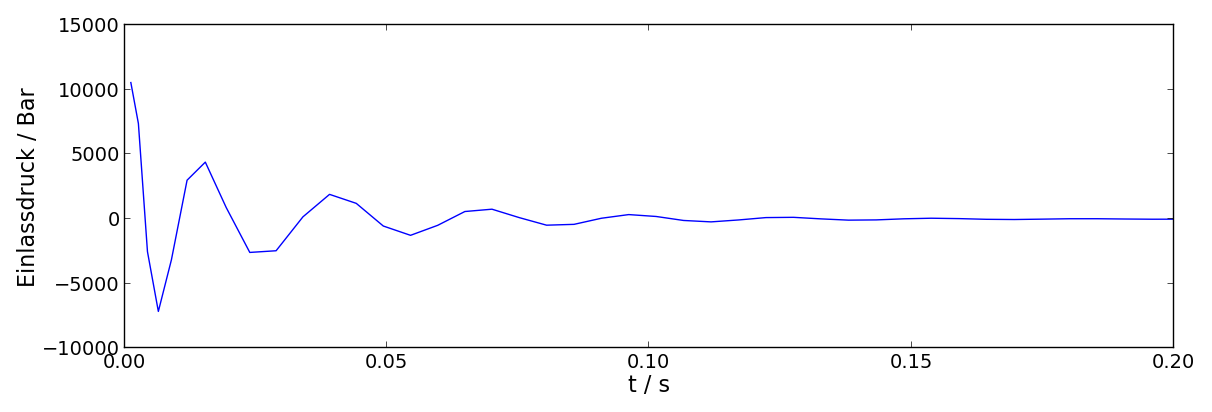
\includegraphics[width=\textwidth]{figures/schwankenderDruck.png}
    \caption{Einlassdruck eines Kapillarrheometers. Die scherratenabhängige Viskosität führt zu starken Oszillationen in der stationären Rechnung, die erst mit der Zeit verschwinden.}
    \label{fig:oszPress}
\end{figure}
%

Um diese Schwingungen zu dämpfen wurde in stationären Berechnungen eine sehr starke Relaxation angewandt. Diese können in \openfoam{} für jedes berechnete Feld separat angegeben werden. Für den Druck $p$ wurden sie im Bereich von $3e-1$ bis $1e-6$, für das Geschwindigkeitsfeld $u$ zwischen $7e-1$ und $1e-4$ gewählt.

In transienten Simulationen kann keine Relaxation angewendet werden. Um die Stabilität der Rechnung trotzdem sicherzustellen, müssen sehr kleine Zeitschritte verwendet werden.
%
\subsection{Konvergenzkriterien}
Die für Simulationen normalerweise verwendeten Residuen des Druck- und Geschwindigkeitfeldes können in Berechnungen mit variabler Viskosität nicht ohne weiteres als Konvergenzkriterium verwendet werden.
Die Kopp\-lung von Geschwindigkeit und Viskosität führt dazu, dass eine Änderung teilweise nur noch in kleinen Regionen stattfindet, diese sich aber durchaus noch über eine grosse Anzahl von Schritten fortsetzen kann.
Daher wurde in der vorliegenden Arbeit statt der Residuen das Verhalten der Be"-ob"-ach"-tungs"-grös"-sen als Konvergenzkriterium verwendet.

Bei Simulationen mit einem Volumenstrom ist dies in dieser Arbeit der Durchschnittsdruck am Einlass:
%
\begin{equation}
    p_\text{\tiny Ave} := \frac{1}{A}\int_{x\in A}p\left( x \right).
\end{equation}
%

In Kapitel \ref{Kapitel:Korrektursimulation} wird beschrieben, wie die Viskosität des Mörtels anhand des Drehmomentes in einem Platte-Platte Rheometer bestimmt wird. In diesen Simulationen ist die beobachtete Grösse nicht ein Druck, sondern das resultierende Drehmoment.\\
Um dieses aus den berechneten Grössen zu extrahieren, wird über die Schubspannung an den vom Nutzer bestimmten Flächen $A_i$ integriert:
%
\begin{equation}
    M = \sum_i \int_{A_i}r\cdot\tau\left( r \right)dA_i,
\end{equation}
wobei 
\begin{equation}
    \tau\left( r \right) = \eta\left( r \right) \cdot \frac{\partial \u\left( r \right)}{\partial \n\left( r \right)}
\end{equation}
die Schubspannung an der Wand und $r$ der Abstand zum Rotationszentrum ist.

Die Auswertung dieser Grössen erfolgt in jedem Iterationsschritt. Die Änderung zwischen zwei Iterationsschritten kann dann als Konvergenzkriterium verwendet werden.\\
Dabei muss darauf geachtet werden, dass nicht nur die erste sondern auch die zweite Ableitung mit einbezogen wird. Andernfalls ist es möglich, dass die Simulation zu früh gestoppt wird, da die beobachteten Grössen teilweise stark schwanken und die erste Ableitung in den Minima und Maxima dieser Schwankungen ebenfalls sehr kleine Werte annimmt.
Die Ableitungen werden mit der Finite Differenzen Methode berechnet:
%%
\begin{eqnarray}
    \label{eq:torqueCalc:fd}
    \dot{x} & = & \frac{1}{2}\left(  x[t+1] - x[t-1] \right), \\
    \ddot{x} & = & \frac{1}{2}\left(  x[t+1] - 2 \cdot x[t] + x[t-1] \right).
\end{eqnarray}

\subsection{Betriebssystem und Hardware}
\label{Kapitel:Hardware}
\openfoam{} kann nicht, beziehungsweise nur mit grossem Aufwand auf Windows installiert werden. Einer der Gründe für diese Einschränkung ist, dass es eine Unterscheidung zwischen Gross- und Kleinschreibung bei Dateinamen benötigt. Die in dieser Arbeit verwendeten Betriebssysteme sind deshalb Linux"~Dis"-tri"-bu"-ti"-o"-nen.

Für kleinere lokale Berechnungen und Testläufe stand ein Laptop zur Verfügung, auf dem Ubuntu 12.04 LTS installiert wurde.
Der Hauptteil der Si"-mu"-la"-ti"-o"-nen wurde aber auf den HPC-Clustern des Swiss National Supercomputing Centre (CSCS) durchgeführt.
Mit dem im Tessin gelegenen Cluster Rothorn stand ein Berechnungsknoten mit 256 CPUs zur Verfügung. Das System ist ein SGI Altix UV 1000, das für Berechnungen einen Ar"-beits"-spei"-cher von 2TB besitzt.
Das Betriebssystem ist SUSE SLES11 SP1.\\
Der Zugang zum Cluster erfolgt über eine 'secure shell' (ssh) Verbindung, mit der man sich über den Zugangsknoten Ela auf Rothorn einloggen kann.

Die visuelle Nachbearbeitung der Resultate wurde ebenfalls beim CSCS gemacht, allerdings nicht auf Rothorn sondern auf einem Dalco SM System, das Eiger genannt wird.\\
Da die Visualisierung eine graphische Benutzeroberfläche benötigt, geschieht die Bedienung nicht über ssh, sondern durch eine 'virtual network computing'-Verbindung, die die Bildschirmausgabe des entfernten Computers auf eine lokale Maschine überträgt und im Gegenzug Maus- und Tastatureingaben zurück sendet.

Diese Art der Auslagerung von Rechnungen auf einen Cluster ermöglicht es, auch grosse und zeitaufwändige Simulationen von einem lokalen Computer aus zu starten und auszuwerten, ohne dass grosse Mengen an Daten hin und her kopiert werden müssen.
